% Birthday problem: exact probability of a shared birthday among n people (solid) and the approximation 1-exp(-n(n-1)/730) (dashed). Generated by a short script.
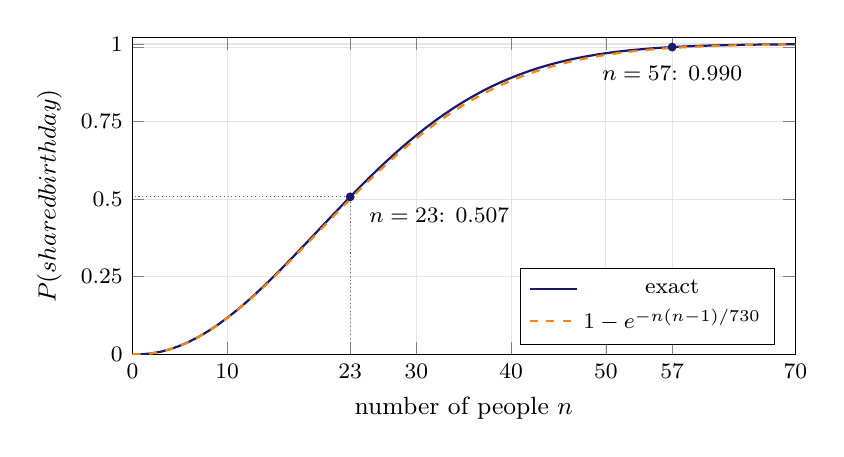
\begin{tikzpicture}
\begin{axis}[width=10cm,height=5.6cm,xmin=0,xmax=70,ymin=0,ymax=1.02,xlabel={number of people $n$},ylabel={$P(\text{shared birthday})$},
  xtick={0,10,23,30,40,50,57,70},ytick={0,0.25,0.5,0.75,0.99,1},yticklabels={$0$,$0.25$,$0.5$,$0.75$,,$1$},grid=major,grid style={black!10},tick label style={font=\footnotesize},label style={font=\small},legend pos=south east,legend style={font=\footnotesize}]
\addplot[MidnightBlue,thick] coordinates {(0,0.00000) (1,0.00000) (2,0.00274) (3,0.00820) (4,0.01636) (5,0.02714) (6,0.04046) (7,0.05624) (8,0.07434) (9,0.09462) (10,0.11695) (11,0.14114) (12,0.16702) (13,0.19441) (14,0.22310) (15,0.25290) (16,0.28360) (17,0.31501) (18,0.34691) (19,0.37912) (20,0.41144) (21,0.44369) (22,0.47570) (23,0.50730) (24,0.53834) (25,0.56870) (26,0.59824) (27,0.62686) (28,0.65446) (29,0.68097) (30,0.70632) (31,0.73045) (32,0.75335) (33,0.77497) (34,0.79532) (35,0.81438) (36,0.83218) (37,0.84873) (38,0.86407) (39,0.87822) (40,0.89123) (41,0.90315) (42,0.91403) (43,0.92392) (44,0.93289) (45,0.94098) (46,0.94825) (47,0.95477) (48,0.96060) (49,0.96578) (50,0.97037) (51,0.97443) (52,0.97800) (53,0.98114) (54,0.98388) (55,0.98626) (56,0.98833) (57,0.99012) (58,0.99166) (59,0.99299) (60,0.99412) (61,0.99509) (62,0.99591) (63,0.99660) (64,0.99719) (65,0.99768) (66,0.99810) (67,0.99844) (68,0.99873) (69,0.99896) (70,0.99916)};
\addlegendentry{exact}
\addplot[BurntOrange,thick,dashed] coordinates {(0,0.00000) (1,0.00000) (2,0.00274) (3,0.00819) (4,0.01630) (5,0.02703) (6,0.04026) (7,0.05591) (8,0.07384) (9,0.09392) (10,0.11599) (11,0.13988) (12,0.16542) (13,0.19241) (14,0.22067) (15,0.24999) (16,0.28019) (17,0.31106) (18,0.34241) (19,0.37406) (20,0.40581) (21,0.43749) (22,0.46894) (23,0.50000) (24,0.53054) (25,0.56041) (26,0.58951) (27,0.61774) (28,0.64499) (29,0.67121) (30,0.69632) (31,0.72028) (32,0.74306) (33,0.76463) (34,0.78497) (35,0.80410) (36,0.82201) (37,0.83873) (38,0.85427) (39,0.86868) (40,0.88199) (41,0.89424) (42,0.90548) (43,0.91575) (44,0.92511) (45,0.93362) (46,0.94132) (47,0.94827) (48,0.95452) (49,0.96012) (50,0.96513) (51,0.96960) (52,0.97356) (53,0.97707) (54,0.98017) (55,0.98290) (56,0.98529) (57,0.98738) (58,0.98921) (59,0.99079) (60,0.99217) (61,0.99335) (62,0.99438) (63,0.99526) (64,0.99601) (65,0.99665) (66,0.99720) (67,0.99766) (68,0.99805) (69,0.99838) (70,0.99866)};
\addlegendentry{$1-e^{-n(n-1)/730}$}
\draw[black!60,densely dotted] (axis cs:23,0)--(axis cs:23,0.5073)--(axis cs:0,0.5073);
\fill[MidnightBlue] (axis cs:23,0.5073) circle (1.6pt);
\node[anchor=west,font=\footnotesize] at (axis cs:24,0.4473) {$n=23$: $0.507$};
\fill[MidnightBlue] (axis cs:57,0.9901) circle (1.6pt);
\node[anchor=north,font=\footnotesize] at (axis cs:57,0.9601) {$n=57$: $0.990$};
\end{axis}
\end{tikzpicture}
